%%%%%%%%%%%%%%%%%%%%%%%%%%%%%%%%%%%%%%%%%%%%%%%%%%%%%%%%%%%%%%%%%%%%%%%%%%%%%
%% INÍCIO CAPÍTULO                                                         %%
%%%%%%%%%%%%%%%%%%%%%%%%%%%%%%%%%%%%%%%%%%%%%%%%%%%%%%%%%%%%%%%%%%%%%%%%%%%%%

\chapter{Levantamento bibliográfico}
\label{cap:2:fundamentacao}

\citacao{%
We can only see a short distance ahead,\\
but we can see plenty there that needs to be done.}
{Alan Mathison Turing}

O entendimento dos fundamentos...

Este Capítulo está organizado da seguinte forma...

% ========================================================================= %
\section{Introdução}
\label{sec:2:introducao}

\citep{brassard1996fundamentals}

% ========================================================================= %
\section{Fundamentação}
\label{sec:2:fundamentacao}

\begin{definicao}[Grafo direcionado com pesos]\label{def:grafo}
\index{grafo!definicao@definição}%
\index{grafo!direcionado com pesos}%
\citep{cormen2009algorithms}
Um grafo direcionado com pesos $G$ é composto por uma tripla ordenada
$G=\langle N, E, \omega \rangle$, onde $N$ representa o conjunto de vértices
(ou nós) do grafo e $E$ o conjunto de arestas ao qual se atribui as seguintes
propriedades:
\begin{inparaenum}[(i)]
\item cada aresta é composta por um par ordenado de nós $(v_1,v_2)$, que
    indica que existe uma ligação saindo do nó $v_1$ em direção ao nó $v_2$ e
\item para cada aresta $e \in E$ existe um peso que é associado por uma
    função $\omega(\cdot)$, que realiza o mapeamento dos pesos de cada aresta
    para um número real, ou seja, $\omega \colon E\mapsto\mathbb{R}$.
\end{inparaenum}
\end{definicao}

\begin{algoritmo}[Cálculo dos graus de entrada e saída de cada nó]
\label{alg:graus}
\index{algoritmo!graus()}%
É possível calcular os graus de entrada e saída de cada nó da rede
de forma iterativa com base na representação por lista de adjacência.

\begin{algorithmic}[1]
\REQUIRE{graus$(L)$}
\STATE\COMMENT{Lista de adjacência $L$ de um grafo direcionado $G=\langle
    N,E\rangle$.}
\STATE $g_\text{in} \leftarrow \text{novo-vetor}(|N|, 0)$
    \COMMENT{Vetor de $|N|$ posições preenchidas com zero.}
\STATE $g_\text{out} \leftarrow \text{novo-vetor}(|N|, 0)$
\FOR{$i$ de $1$ até $|N|$}
    \FORALL{$(v_j,p) \in L[i]$}
        \STATE\COMMENT{Nó adjacente $v_j$ e peso $p$ da aresta.}
        \STATE $g_\text{out}[i] \leftarrow g_\text{out}[i] + 1$
        \STATE $g_\text{in}[j] \leftarrow g_\text{in}[j] + 1$
    \ENDFOR
\ENDFOR
\RETURN $\langle g_\text{in}, g_\text{out} \rangle$
\COMMENT{Vetores com os graus de entrada e saída de cada nó da rede.}
\end{algorithmic}
Considera-se que os vetores $g_\text{in}$ e $g_\text{out}$ são indexados a
partir de 1.
A complexidade do algoritmo é da ordem de 
$\Theta(n\operatorname{E}\{\mathcal{G}^\text{out}\})$ em tempo e $\Theta(n)$
em memória.
\end{algoritmo}

% ========================================================================= %
\section{Objetivos específicos}
\label{sec:2:objetivos}


% ========================================================================= %
\section{Metodologia}
\label{sec:2:metodologia}

O procedimento metodológico utilizado no desenvolvimento deste trabalho
possui uma abordagem dividida em 5 estágios.
Esses estágios são ordenados em uma sequência em que é permitida uma evolução
com ciclos, cuja relação é descrita na Figura~\ref{fig:metodologia}.

\begin{figure}[ht]
\index{metodologia!procedimento}
\centering
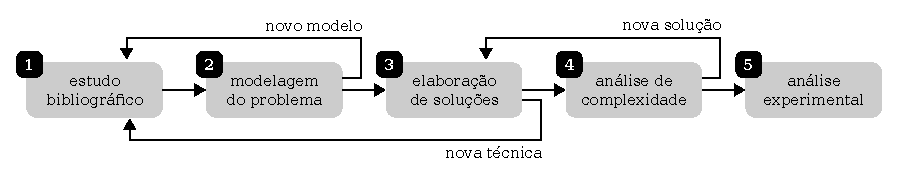
\includegraphics[scale=1]{image/metodologia}
\caption[Ilustração do procedimento metodológico]
    {Ilustração do procedimento metodológico adotado no desenvolvimento deste
    trabalho.
    O processo foi divido em 5 estágios:
    (1) estudo bibliográfico para fundamentar o desenvolvimento de modelos
        representativos do problema;
    (2) modelagem do problema para servir de referência para a elaboração de
        soluções que, se identificadas como inadequadas, podem remeter
        novamente ao estudo bibliográfico;
    (3) elaboração de soluções algorítmicas que serão avaliadas nos próximos
        estágios;
    (4) análise de complexidade das soluções que, quando ineficientes, podem
        remeter a elaboração de uma nova solução e
    (5) análise experimental dos resultados teóricos.}
\label{fig:metodologia}
\end{figure}

A seguir, cada um dos estágios do procedimento metodológico apresentado na
Figura~\ref{fig:metodologia} é descrito.
Na descrição de cada estágio, são considerados, além de seu objetivo, as
possibilidades de evolução de acordo com a ilustração apresentada.

\begin{compactenum}
\item {\bf Estudo bibliográfico}: consiste na busca por bibliografia de
    referência e soluções anteriores para o problema considerado, incluindo
    soluções para problemas similares ou logicamente equivalentes.
    Em relação à evolução temos que:
    \begin{compactenum}[(i)]
    \item o estudo inicial pode levar a um ciclo de busca por soluções que,
        por sua vez, pode remeter ao estudo bibliográfico de outros trabalhos
        e
    \item dado que a bibliografia levantada é tida como definitiva, o próximo
        estágio a ser considerado é o da criação de um modelo para o problema
        que possa ser utilizado na elaboração de soluções.
    \end{compactenum}
\item {\bf Modelagem do problema}: com base no referencial teórico construído
    no primeiro estágio deve-se criar um modelo matemático que represente o
    problema de forma eficaz.
    Em relação à evolução desse estágio têm-se três opções:
    \begin{compactenum}[(i)]
    \item passar para o estágio de elaboração de soluções quando o modelo é
        eficaz para o problema em questão;
    \item estender a modelagem ao se verificar uma deficiência na abordagem
        encontrada na literatura e
    \item possivelmente, quando a necessidade de extensão ocorre, deve-se
        recorrer novamente ao estudo bibliográfico, pois essas extensões
        devem ser cuidadosamente projetadas e validadas.
    \end{compactenum}
\item {\bf Elaboração de soluções}: a partir do modelo criado no estágio
    anterior, é possível elaborar soluções algorítmicas e aplicar métodos de
    otimização a fim de solucionar o problema redefinido com base no modelo
    matemático construído;
    Em relação à evolução desse estágio têm-se três opções:
    \begin{compactenum}[(i)]
    \item passar para o estágio de análise de complexidade da solução, seja
        essa complexidade associada à necessidade de recursos de tempo ou de
        memória;
    \item estender a solução para subproblemas do modelo a fim de verificar
        propriedades que caracterizam e subsidiam a formação de hipóteses e
    \item possivelmente, quando a necessidade de uma nova técnica ocorre,
        deve-se recorrer novamente ao estudo bibliográfico.
    \end{compactenum}
\item {\bf Análise de complexidade}: cada solução projetada tem um custo de
    implementação associado.
    A princípio, este custo não deve inviabilizar a utilização da solução em
    termos de tempo e memória, dentre outros recursos, necessários para
    resolver o problema em questão.
    Em relação à evolução temos que:
    \begin{compactenum}[(i)]
    \item se as complexidades envolvidas satisfizerem os requisitos, então
        evolui-se para o estágio de implementação das soluções de forma
        integrada e
    \item se a complexidade for proibitiva, é necessário voltar ao estágio de
        elaboração para construção de uma outra solução.
    \end{compactenum}
\item {\bf Análise experimental}: se o estágio de análise de complexidade
    fomenta a utilização da solução proposta, deve-se realizar experimentos
    com dados reais para validar a solução, ou aplicá-las à instâncias do
    modelo a fim de extrair conjecturas acerca das propriedades do modelo que
    indiquem a validade da solução.
\end{compactenum}

%%%%%%%%%%%%%%%%%%%%%%%%%%%%%%%%%%%%%%%%%%%%%%%%%%%%%%%%%%%%%%%%%%%%%%%%%%%%%
%% FIM CAPÍTULO                                                            %%
%%%%%%%%%%%%%%%%%%%%%%%%%%%%%%%%%%%%%%%%%%%%%%%%%%%%%%%%%%%%%%%%%%%%%%%%%%%%%
